\section{Introduction}
Blockchain technology has revolutionized digital trust and decentralized applications, but this innovation has been accompanied by significant security challenges. The rapid proliferation of smart contracts, DeFi protocols, and cross-chain infrastructure has created a complex attack surface that traditional security frameworks struggle to address systematically. This paper presents B-SAFE, a comprehensive framework for blockchain security assessment that provides a unified approach to understanding, classifying, and quantifying security risks across the entire blockchain ecosystem.

The B-SAFE framework addresses the critical need for systematic security analysis in blockchain systems by introducing a five-layer reference architecture that captures the complete attack surface. Our methodology enables reproducible security assessment through standardized data collection, incident labeling, and risk quantification, providing actionable insights for researchers, practitioners, and policymakers.

\begin{figure}[H]
\centering
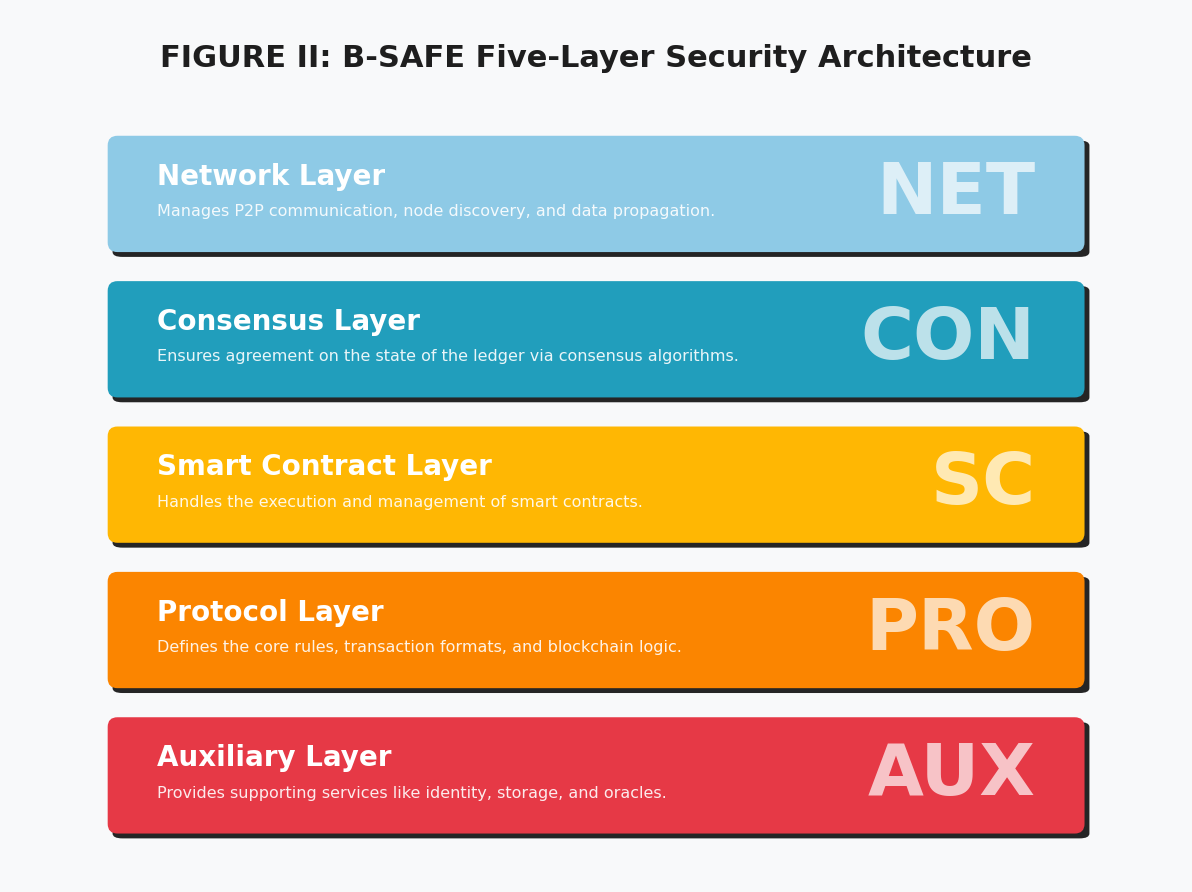
\includegraphics[width=0.4\textwidth]{../figure/fig2.png}
\caption{Five-layer B-SAFE architecture showing the hierarchical organization of blockchain security threats: Network (NET), Consensus (CON), Smart Contract (SC), Protocol (PRO), and Auxiliary (AUX) layers with cross-layer dependencies indicated by arrows.}
\label{fig:five_layer_architecture}
\end{figure}